\documentclass[
  coursetitle={Cómputo Nube y Tecnologías Emergentes},
  coursehours={96},
  coursedate={Verano 2026},
  doctype={Tutorial},
  otherlangs={english},
  authorname={Lázaro},
  authorsurname={Bustio-Martínez},
  authortitle={PhD},
  role={Profesor Investigador},
  email={lbustio@inaoe.mx},
  phone={5559504000},
  ext={7459},
  institution={Instituto Nacional de Astrofísica, Óptica y Electrónica (INAOE)},
  department={Maestría en Ciencias en Tecnologías de Seguridad},
  address={Luis Enrique Erro 1, Sta. Ma. Tonantzintla, San Andrés Cholula, CP 72840, Puebla, México},
  margin={0.5in}
]{../../../lbustio_lecture_notes}

\usepackage[utf8]{inputenc}
\usepackage[T1]{fontenc}
\usepackage{array}
\usepackage{tabularx}
\usepackage{enumitem}
\usepackage{longtable}
\usepackage{booktabs}
\usepackage{url}
\usepackage{listings}
\usepackage{xcolor}
\usepackage{graphicx}
\usepackage{tcolorbox}
\usepackage{verbatim}
\usepackage{tikz}
\usetikzlibrary{arrows.meta,backgrounds,fit,positioning}

\begingroup
\catcode`\:=\active
\gdef:{\string:}
\endgroup

\definecolor{lightgray}{rgb}{0.97, 0.97, 0.97}
\definecolor{darkblue}{rgb}{0, 0, 0.6}
\definecolor{gcpblue}{HTML}{4285F4}
\definecolor{gcpgreen}{HTML}{34A853}
\definecolor{gcpyellow}{HTML}{FBBC04}
\definecolor{gcpred}{HTML}{EA4335}
\definecolor{softgray}{HTML}{F5F7FA}
\definecolor{androidgreen}{HTML}{3DDC84}
\definecolor{androiddark}{HTML}{073042}

\lstset{
  backgroundcolor=\color{lightgray},
  basicstyle=\ttfamily\small,
  breaklines=true,
  frame=single,
  columns=fullflexible,
  showstringspaces=false,
  commentstyle=\color{gray},
  keywordstyle=\color{darkblue},
  inputencoding=utf8,
  extendedchars=true,
  literate={á}{{\'a}}1 {é}{{\'e}}1 {í}{{\'i}}1 {ó}{{\'o}}1 {ú}{{\'u}}1 {ñ}{{\~n}}1
           {Á}{{\'A}}1 {É}{{\'E}}1 {Í}{{\'I}}1 {Ó}{{\'O}}1 {Ú}{{\'U}}1 {Ñ}{{\~N}}1
}

\setlist[itemize]{topsep=0.3em,itemsep=0.2em}
\setlist[enumerate]{topsep=0.3em,itemsep=0.2em}

\tikzset{
  gcpstage/.style={
    draw=gcpblue,
    fill=gcpblue!8,
    rounded corners=4pt,
    very thick,
    align=center,
    text width=0.62\textwidth,
    minimum height=1.15cm,
    inner sep=7pt
  },
  gcpstage2/.style={
    gcpstage,
    draw=gcpgreen!80!black,
    fill=gcpgreen!9
  },
  gcpstage3/.style={
    gcpstage,
    draw=gcpred,
    fill=gcpred!7
  },
  gcpstage4/.style={
    gcpstage,
    draw=androiddark,
    fill=androiddark!7
  },
  flowarrow/.style={
    -{Latex[length=3mm,width=2mm]},
    thick,
    draw=darkblue
  }
}

\begin{document}

\IberoCover

\section{Propósito de la práctica}

En la práctica anterior se desarrolló la parte analítica del problema: se tomó un dataset de aplicaciones Android, se representaron las APKs mediante vectores binarios de permisos, se entrenó un modelo de aprendizaje automático y se generó un artefacto reutilizable en formato \texttt{.joblib}.

Ese análisis responde una pregunta de investigación:

\begin{quote}
\textit{¿Los permisos declarados en el manifiesto Android contienen información suficiente para clasificar una aplicación como benigna o maliciosa?}
\end{quote}

En esta práctica se dará el siguiente paso: convertir ese análisis en una aplicación desplegada en la nube.

El objetivo no es volver a entrenar el modelo. El objetivo es tomar una aplicación que ya funciona localmente y publicarla como un servicio web en Google Cloud Platform usando:

\begin{itemize}
  \item \textbf{Cloud Build}, para construir la imagen del contenedor en la nube.
  \item \textbf{Artifact Registry}, para almacenar la imagen del contenedor.
  \item \textbf{Cloud Run}, para ejecutar la aplicación como servicio serverless.
  \item \textbf{gcloud CLI}, para controlar el despliegue desde la terminal.
\end{itemize}

Al finalizar, el estudiante tendrá una URL pública de Cloud Run donde podrá cargar una APK pequeña y obtener una predicción automática del modelo.

\section{Historia técnica del problema}

Cuando una aplicación funciona en la computadora local, normalmente se ejecuta bajo condiciones controladas:

\begin{itemize}
  \item el código está en disco local;
  \item el modelo \texttt{.joblib} está disponible en una ruta conocida;
  \item Flask puede escuchar en \texttt{127.0.0.1};
  \item el navegador y el backend están en la misma máquina;
  \item los archivos se suben directamente sin restricciones fuertes de infraestructura.
\end{itemize}

En la nube eso cambia. Cloud Run no ejecuta la aplicación como un script normal en una computadora personal. Cloud Run ejecuta un contenedor. Ese contenedor debe cumplir un contrato mínimo:

\begin{itemize}
  \item debe escuchar en \texttt{0.0.0.0}, no en \texttt{127.0.0.1};
  \item debe usar el puerto indicado por la variable de entorno \texttt{PORT};
  \item debe incluir todas sus dependencias;
  \item debe contener el código necesario para arrancar la aplicación;
  \item debe tener disponible el modelo entrenado;
  \item debe responder dentro de los límites de Cloud Run.
\end{itemize}

Por eso el despliegue no consiste simplemente en ``subir el código''. Hay que empaquetar la aplicación, construir una imagen, almacenarla en un registro y desplegarla como servicio.

\section{Arquitectura de la solución}

\begin{center}
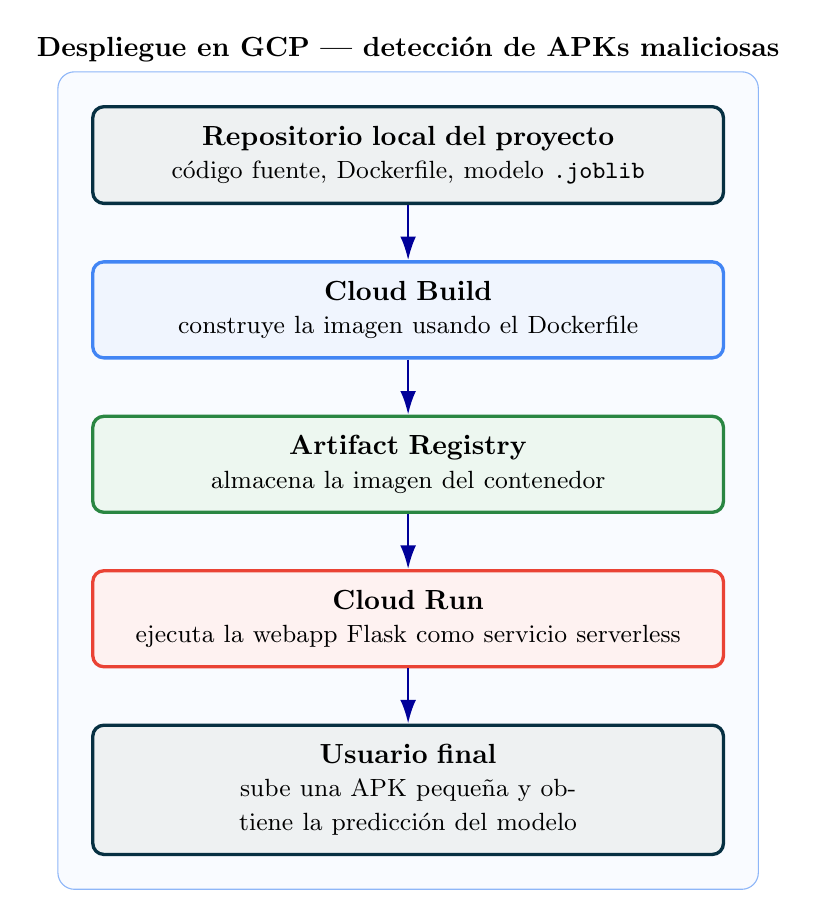
\begin{tikzpicture}[node distance=0.7cm]
    \node[gcpstage4] (repo) {
        \textbf{Repositorio local del proyecto}\\
        \small código fuente, Dockerfile, modelo \texttt{.joblib}
    };
    \node[gcpstage, below=of repo] (build) {
        \textbf{Cloud Build}\\
        \small construye la imagen usando el Dockerfile
    };
    \node[gcpstage2, below=of build] (registry) {
        \textbf{Artifact Registry}\\
        \small almacena la imagen del contenedor
    };
    \node[gcpstage3, below=of registry] (run) {
        \textbf{Cloud Run}\\
        \small ejecuta la webapp Flask como servicio serverless
    };
    \node[gcpstage4, below=of run] (user) {
        \textbf{Usuario final}\\
        \small sube una APK pequeña y obtiene la predicción del modelo
    };

    \draw[flowarrow] (repo) -- (build);
    \draw[flowarrow] (build) -- (registry);
    \draw[flowarrow] (registry) -- (run);
    \draw[flowarrow] (run) -- (user);

    \begin{scope}[on background layer]
        \node[
            draw=gcpblue!60,
            fill=gcpblue!3,
            rounded corners=6pt,
            inner sep=12pt,
            fit=(repo)(build)(registry)(run)(user),
            label={[font=\bfseries]above:Despliegue en GCP --- detección de APKs maliciosas}
        ] {};
    \end{scope}
\end{tikzpicture}

\small\textbf{Figura:} Flujo de despliegue desde el repositorio local hasta el servicio Cloud Run.
\end{center}

La aplicación desplegada contiene código backend, código frontend, modelo entrenado, parser de manifiestos Android, dependencias Python, rutas Flask e interfaz web. La práctica usa despliegue directo por HTTP, por lo que solo se aceptarán APKs pequeñas.

\section{Restricción de tamaño de APK}
\label{sec-restriccion-tamano}

Cloud Run tiene un límite de 32 MiB para solicitudes HTTP/1. Si el archivo enviado es demasiado grande, Google Frontend rechaza la petición antes de que llegue a Flask.

\textbf{En esta práctica se trabajará con APKs menores de 30 MiB.}

No se deben usar APKs grandes como:

\begin{lstlisting}
WhatsApp.xapk      82.28 MB
homestar_apk.apk   61.75 MB
\end{lstlisting}

Con archivos de ese tamaño, Cloud Run devuelve:

\begin{lstlisting}
HTTP/1.1 413 Request Entity Too Large
\end{lstlisting}

y la interfaz puede mostrar un error como:

\begin{lstlisting}
Unexpected token '<', "<html><hea"... is not valid JSON
\end{lstlisting}

Ese error significa que el frontend esperaba JSON pero recibió una página HTML de error generada por Google Frontend.

Para esta práctica, la solución correcta es usar APKs pequeñas. El manejo de APKs grandes requiere otra arquitectura, normalmente basada en Cloud Storage, pero esa arquitectura no forma parte de esta práctica.

\section{Requisitos previos}

Antes de iniciar, el estudiante debe tener:

\begin{itemize}
  \item cuenta de Google Cloud;
  \item proyecto de GCP creado;
  \item facturación habilitada;
  \item gcloud CLI instalado;
  \item repositorio del proyecto disponible localmente;
  \item modelo entrenado previamente;
  \item una APK de prueba menor de 30 MiB.
\end{itemize}

\begin{tcolorbox}[title=Docker Desktop no es obligatorio]
La imagen se construirá en la nube usando Cloud Build. Esto evita depender de Docker local, WSL, Hyper-V, virtualización en BIOS o problemas de Docker Desktop en Windows.
\end{tcolorbox}

\section{Estructura del proyecto}
\label{sec-estructura}

Desde la raíz del proyecto deben existir, al menos, estos archivos y carpetas:

\begin{lstlisting}
malware_apk_detection/
  requirements.txt
  Dockerfile
  .dockerignore
  backend/
    android_threat_analyzer/
      web.py
      model.py
      analysis.py
      manifest.py
  frontend_webapp/
    app.py
    static/
      app.js
      styles.css
    templates/
      index.html
  models/
    android_permission_best_model.joblib
  testapk/
    small_test.apk
\end{lstlisting}

Antes de desplegar, verificar que existen los elementos críticos:

\begin{lstlisting}
Get-ChildItem requirements.txt
Get-ChildItem frontend_webapp\app.py
Get-ChildItem models\android_permission_best_model.joblib
\end{lstlisting}

\textbf{Resultado esperado:} los tres archivos existen. Si alguno falta, el despliegue no debe continuar.

\section{Crear el archivo \texttt{.dockerignore}}

En la raíz del proyecto, crear el archivo \texttt{.dockerignore} con el siguiente contenido:

\begin{lstlisting}
.git
__pycache__
*.pyc
*.pyo
logs/
testapk/
notebooks/
references/
biblio/
environment.yml
\end{lstlisting}

Este archivo evita que el contenedor incluya archivos innecesarios.

\begin{tcolorbox}[title=No excluir la carpeta models/]
La carpeta \texttt{models/} no debe aparecer en \texttt{.dockerignore}. El modelo \texttt{.joblib} debe quedar dentro de la imagen para que Cloud Run pueda cargarlo. Si se excluye por accidente, el contenedor arrancará pero el endpoint \texttt{/health} mostrará \texttt{model\_loaded: false}.
\end{tcolorbox}

\textbf{Resultado esperado:} la imagen será más ligera y no incluirá notebooks, referencias ni APKs de prueba. El modelo entrenado sí quedará empaquetado.

\section{Crear el Dockerfile}

En la raíz del proyecto, crear el archivo \texttt{Dockerfile} con el siguiente contenido:

\begin{lstlisting}
FROM python:3.11-slim

WORKDIR /app

COPY requirements.txt .

RUN pip install --no-cache-dir -r requirements.txt

COPY . .

ENV APK_DETECTOR_HOST=0.0.0.0

CMD ["sh", "-c", "APK_DETECTOR_PORT=${PORT:-8080} python -m frontend_webapp.app"]
\end{lstlisting}

Cada instrucción cumple una función específica:

\begin{description}
  \item[\texttt{FROM python:3.11-slim}]
    Define la imagen base. Se usa Python 3.11 en una versión ligera.
  \item[\texttt{WORKDIR /app}]
    Define \texttt{/app} como carpeta de trabajo dentro del contenedor.
  \item[\texttt{COPY requirements.txt .}]
    Copia primero el archivo de dependencias. Docker puede reutilizar esta capa si el código cambia pero las dependencias no.
  \item[\texttt{RUN pip install}]
    Instala las dependencias sin almacenar caché de pip, lo que reduce el tamaño de la imagen.
  \item[\texttt{COPY . .}]
    Copia el código completo del proyecto al contenedor, incluyendo el modelo \texttt{.joblib}.
  \item[\texttt{ENV APK\_DETECTOR\_HOST=0.0.0.0}]
    Hace que Flask escuche en todas las interfaces de red del contenedor. Esto es \textbf{obligatorio} en Cloud Run según la documentación oficial. Si la aplicación escucha solo en \texttt{127.0.0.1}, Cloud Run no podrá enrutar tráfico hacia ella.
  \item[\texttt{CMD}]
    Cloud Run inyecta la variable de entorno \texttt{PORT}. La aplicación usa \texttt{APK\_DETECTOR\_PORT}. El comando en forma de shell toma el puerto de Cloud Run y lo pasa a la aplicación. Si \texttt{PORT} no está definida, usa \texttt{8080} como valor por defecto.
\end{description}

\textbf{Resultado esperado:} el contenedor podrá arrancar en Cloud Run; Flask escuchará en el puerto correcto; el modelo \texttt{.joblib} estará disponible dentro de \texttt{/app/models/}.

\section{Configurar el proyecto de GCP}

Abrir PowerShell y ejecutar:

\begin{lstlisting}
$PROJECT_ID = "cloud-computing-cybersec-inaoe"

gcloud auth login

gcloud config set project $PROJECT_ID
\end{lstlisting}

Verificar el proyecto activo:

\begin{lstlisting}
gcloud config get-value project
\end{lstlisting}

\textbf{Resultado esperado:}

\begin{lstlisting}
cloud-computing-cybersec-inaoe
\end{lstlisting}

Si aparece otro proyecto, no continuar.

\section{Habilitar APIs necesarias}

Ejecutar:

\begin{lstlisting}
gcloud services enable `
  run.googleapis.com `
  cloudbuild.googleapis.com `
  artifactregistry.googleapis.com
\end{lstlisting}

Verificar:

\begin{lstlisting}
gcloud services list --enabled --filter="name:(run.googleapis.com OR cloudbuild.googleapis.com OR artifactregistry.googleapis.com)"
\end{lstlisting}

\textbf{Resultado esperado:}

\begin{lstlisting}
artifactregistry.googleapis.com
cloudbuild.googleapis.com
run.googleapis.com
\end{lstlisting}

\begin{description}
  \item[\texttt{run.googleapis.com}] Permite usar Cloud Run.
  \item[\texttt{cloudbuild.googleapis.com}] Permite construir imágenes en la nube.
  \item[\texttt{artifactregistry.googleapis.com}] Permite almacenar imágenes Docker en Artifact Registry.
\end{description}

\begin{tcolorbox}[title=Container Registry está deprecado]
No usar \texttt{containerregistry.googleapis.com} como ruta principal. Container Registry está deprecado según la documentación oficial de Google Cloud. La práctica usa Artifact Registry, que es el servicio actual y recomendado.
\end{tcolorbox}

\section{Crear repositorio en Artifact Registry}

Artifact Registry guardará la imagen del contenedor.

\begin{lstlisting}
$REGION = "us-central1"
$REPO = "malware-apk-repo"

gcloud artifacts repositories create $REPO `
  --repository-format=docker `
  --location=$REGION `
  --description="Repositorio Docker para la práctica de detección de APKs maliciosas"
\end{lstlisting}

Verificar:

\begin{lstlisting}
gcloud artifacts repositories list --location=us-central1
\end{lstlisting}

\textbf{Resultado esperado:}

\begin{lstlisting}
REPOSITORY: malware-apk-repo
FORMAT: DOCKER
MODE: STANDARD_REPOSITORY
LOCATION: us-central1
\end{lstlisting}

Si el repositorio ya existe, no es necesario crearlo de nuevo.

\section{Construir la URI de la imagen}

La convención actual de Artifact Registry para la URI de una imagen es:

\begin{lstlisting}
LOCATION-docker.pkg.dev/PROJECT_ID/REPOSITORY/IMAGE_NAME:TAG
\end{lstlisting}

Desde PowerShell, definir las variables y construir la URI:

\begin{lstlisting}
$PROJECT_ID = "cloud-computing-cybersec-inaoe"
$REGION = "us-central1"
$REPO = "malware-apk-repo"
$IMAGE = "malware-apk-detector"
$IMAGE_URI = "${REGION}-docker.pkg.dev/${PROJECT_ID}/${REPO}/${IMAGE}:latest"

Write-Host $IMAGE_URI
\end{lstlisting}

\textbf{Resultado esperado:}

\begin{lstlisting}
us-central1-docker.pkg.dev/cloud-computing-cybersec-inaoe/malware-apk-repo/malware-apk-detector:latest
\end{lstlisting}

\begin{tcolorbox}[title=Advertencia: interpolación de variables en PowerShell]
En PowerShell, no escribir la URI sin llaves delimitadoras. La sintaxis \texttt{\$REGION-docker.pkg.dev/...} puede producir resultados inesperados porque PowerShell puede no delimitar correctamente el nombre de la variable junto al carácter \texttt{-}.

Usar siempre llaves: \texttt{\$\{REGION\}}, \texttt{\$\{PROJECT\_ID\}}, \texttt{\$\{REPO\}}, \texttt{\$\{IMAGE\}}. Si \texttt{\$IMAGE\_URI} no está bien construida, el siguiente paso fallará con \texttt{invalid reference format}.
\end{tcolorbox}

\section{Construir la imagen con Cloud Build}

Ubicarse en la raíz del proyecto (donde está el Dockerfile) y ejecutar:

\begin{lstlisting}
gcloud builds submit --tag $IMAGE_URI
\end{lstlisting}

Internamente ocurre lo siguiente:

\begin{enumerate}
  \item gcloud comprime el proyecto.
  \item Sube temporalmente el código a Cloud Storage.
  \item Cloud Build lee el Dockerfile.
  \item Cloud Build descarga la imagen base \texttt{python:3.11-slim}.
  \item Instala las dependencias de \texttt{requirements.txt}.
  \item Copia el código y el modelo al contenedor.
  \item Construye la imagen.
  \item Publica la imagen en Artifact Registry.
\end{enumerate}

Durante el proceso se verá una salida similar a:

\begin{lstlisting}
Creating temporary archive...
Uploading tarball...
FETCHSOURCE
BUILD
Step 1/7 : FROM python:3.11-slim
Step 2/7 : WORKDIR /app
Step 3/7 : COPY requirements.txt .
Step 4/7 : RUN pip install --no-cache-dir -r requirements.txt
Step 5/7 : COPY . .
Step 6/7 : ENV APK_DETECTOR_HOST=0.0.0.0
Step 7/7 : CMD [...]
Successfully built ...
Successfully tagged ...
PUSH
DONE
STATUS: SUCCESS
\end{lstlisting}

\textbf{Resultado esperado:}

\begin{lstlisting}
STATUS: SUCCESS
\end{lstlisting}

Si aparece \texttt{invalid reference format}, la variable \texttt{\$IMAGE\_URI} está mal construida. Revisar el paso anterior y asegurarse de usar llaves en la interpolación.

\section{Verificar imagen en Artifact Registry}

Ejecutar:

\begin{lstlisting}
gcloud artifacts docker images list `
  us-central1-docker.pkg.dev/cloud-computing-cybersec-inaoe/malware-apk-repo
\end{lstlisting}

\textbf{Resultado esperado:}

\begin{lstlisting}
malware-apk-detector
\end{lstlisting}

Esto confirma que la imagen existe y puede ser usada por Cloud Run.

\section{Desplegar la aplicación en Cloud Run}

Ejecutar:

\begin{lstlisting}
$PROJECT_ID = "cloud-computing-cybersec-inaoe"
$REGION = "us-central1"
$REPO = "malware-apk-repo"
$IMAGE = "malware-apk-detector"
$SERVICE = "malware-apk-detector"
$IMAGE_URI = "${REGION}-docker.pkg.dev/${PROJECT_ID}/${REPO}/${IMAGE}:latest"

gcloud run deploy $SERVICE `
  --image $IMAGE_URI `
  --region $REGION `
  --platform managed `
  --allow-unauthenticated `
  --memory 1Gi `
  --timeout 300
\end{lstlisting}

Cada parámetro cumple una función:

\begin{description}
  \item[\texttt{--image}]
    Indica qué imagen de Artifact Registry se va a ejecutar.
  \item[\texttt{--region}]
    Define la región donde se desplegará el servicio.
  \item[\texttt{--platform managed}]
    Indica que se usará Cloud Run administrado.
  \item[\texttt{--allow-unauthenticated}]
    Permite acceder a la webapp sin autenticación. Para una práctica de clase es aceptable porque evita gestionar tokens o IAM de usuarios finales. En producción real no debe usarse sin análisis de seguridad.
  \item[\texttt{--memory 1Gi}]
    Asigna 1 GiB de memoria. Se usa más de 512 MiB porque la aplicación carga bibliotecas pesadas como Pandas, NumPy, SciPy y Scikit-Learn.
  \item[\texttt{--timeout 300}]
    Permite hasta 300 segundos por request. Esto evita cortes tempranos durante análisis más lentos.
\end{description}

\textbf{Resultado esperado:}

\begin{lstlisting}
Service [malware-apk-detector] revision [...] has been deployed and is serving 100 percent of traffic.
Service URL: https://malware-apk-detector-XXXXXXXXXXXX.us-central1.run.app
\end{lstlisting}

Guardar la URL del servicio. Será la URL pública de la aplicación.

\section{Verificar que la aplicación responde}

Los comandos siguientes usan la URL de ejemplo generada por Cloud Run.

Verificar la página principal:

\begin{lstlisting}
curl.exe -I https://malware-apk-detector-626352904706.us-central1.run.app
\end{lstlisting}

\textbf{Resultado esperado:}

\begin{lstlisting}
HTTP/2 200
\end{lstlisting}

Verificar el endpoint de salud:

\begin{lstlisting}
curl.exe https://malware-apk-detector-626352904706.us-central1.run.app/health
\end{lstlisting}

\textbf{Resultado esperado:}

\begin{lstlisting}
{
  "log_file": "/app/logs/webapp.log",
  "model_loaded": true,
  "model_path": "/app/models/android_permission_best_model.joblib",
  "status": "ok"
}
\end{lstlisting}

\begin{tcolorbox}[title=Interpretación del health check]
\texttt{model\_loaded: true} significa que el modelo \texttt{.joblib} fue cargado correctamente dentro del contenedor. \texttt{status: ok} significa que el backend está operativo. Si \texttt{model\_loaded} es \texttt{false}, verificar que \texttt{models/} no está excluido en \texttt{.dockerignore} y reconstruir la imagen.
\end{tcolorbox}

\section{Revisar logs de la aplicación}

La aplicación incluye un endpoint de logs:

\begin{lstlisting}
curl.exe https://malware-apk-detector-626352904706.us-central1.run.app/logs?lines=80
\end{lstlisting}

También se pueden leer logs desde Google Cloud:

\begin{lstlisting}
gcloud logging read `
  'resource.type="cloud_run_revision" AND resource.labels.service_name="malware-apk-detector"' `
  --project="cloud-computing-cybersec-inaoe" `
  --limit=20 `
  --format="table(timestamp,severity,textPayload)"
\end{lstlisting}

\textbf{Resultado esperado en logs internos:}

\begin{lstlisting}
Cargando modelo desde /app/models/android_permission_best_model.joblib
Artefacto cargado model_type=Pipeline features=330
Modelo cargado correctamente
Iniciando Flask host=0.0.0.0 port=8080
GET / status=200
GET /health status=200
\end{lstlisting}

Esto confirma que el contenedor arrancó, Flask escucha en \texttt{0.0.0.0}, Cloud Run inyectó el puerto correcto, el modelo fue cargado y la interfaz web está sirviendo archivos estáticos.

\section{Probar análisis de una APK pequeña}

Verificar el tamaño de las APKs disponibles:

\begin{lstlisting}
Get-ChildItem testapk | Select-Object Name,@{Name="Size_MB";Expression={[math]::Round($_.Length / 1MB, 2)}} | Sort-Object Size_MB -Descending
\end{lstlisting}

\textbf{Ejemplo esperado:}

\begin{lstlisting}
small_test.apk     12.40
\end{lstlisting}

Enviar la APK al endpoint \texttt{/analyze}:

\begin{lstlisting}
$URL = "https://malware-apk-detector-626352904706.us-central1.run.app/analyze"
$APK = "testapk\small_test.apk"

curl.exe -i -X POST `
  -F "apk=@$APK" `
  $URL
\end{lstlisting}

\textbf{Resultado esperado:}

\begin{lstlisting}
HTTP/2 200
content-type: application/json

{
  "filename": "small_test.apk",
  "prediction": "benigna",
  "malware_probability": 0.1234,
  "risk_score": 12,
  "permissions": [...]
}
\end{lstlisting}

El contenido exacto depende de la APK y del modelo entrenado.

\section{Probar desde el navegador}

Abrir la URL del servicio Cloud Run en el navegador. Seleccionar una APK menor de 30 MiB y presionar el botón de análisis.

\textbf{Resultado esperado:}

\begin{itemize}
  \item la interfaz acepta el archivo;
  \item el backend analiza el manifiesto Android;
  \item el modelo genera la predicción;
  \item la respuesta aparece como resultado en pantalla;
  \item no aparece error de JSON.
\end{itemize}

\section{Error conocido: respuesta inesperada en lugar de JSON}

Si aparece el siguiente error en la interfaz:

\begin{lstlisting}
Unexpected token '<', "<html><hea"... is not valid JSON
\end{lstlisting}

significa que el frontend intentó interpretar como JSON una respuesta que en realidad era HTML de error. La causa más común en esta práctica es:

\begin{lstlisting}
HTTP/1.1 413 Request Entity Too Large
\end{lstlisting}

Esto ocurre cuando se intenta subir una APK demasiado grande. Para diagnosticar desde la consola:

\begin{lstlisting}
$URL = "https://malware-apk-detector-626352904706.us-central1.run.app/analyze"
$APK = "testapk\homestar_apk.apk"

curl.exe -i -X POST `
  -F "apk=@$APK" `
  $URL
\end{lstlisting}

\textbf{Respuesta típica con archivo grande:}

\begin{lstlisting}
HTTP/1.1 413 Request Entity Too Large
content-type: text/html; charset=UTF-8
server: Google Frontend

<html>
<head>
<title>413 Request Entity Too Large</title>
</head>
<body>
<h1>Error: Request Entity Too Large</h1>
<h2>Your client issued a request that was too large.</h2>
</body>
</html>
\end{lstlisting}

\begin{tcolorbox}[title=Interpretación del error 413]
La petición no llegó a Flask. La rechazó Google Frontend antes. El backend no puede manejar ese error porque nunca lo recibe. Aumentar la memoria del servicio no soluciona el problema. Aumentar el timeout tampoco. El archivo debe ser menor de 30 MiB. Este es un límite de la infraestructura HTTP/1 de Cloud Run, no de la aplicación.
\end{tcolorbox}

\section{Validación de tamaño en el frontend}

Para evitar que el usuario suba archivos demasiado grandes, agregar una validación en \texttt{frontend\_webapp/static/app.js}, antes de la llamada a \texttt{fetch("/analyze", ...)}:

\begin{lstlisting}
const MAX_APK_SIZE_MB = 30;
const MAX_APK_SIZE_BYTES = MAX_APK_SIZE_MB * 1024 * 1024;

if (file.size > MAX_APK_SIZE_BYTES) {
  showError(
    `El archivo pesa ${(file.size / 1024 / 1024).toFixed(2)} MB. ` +
    `Para esta práctica en Cloud Run solo se aceptan APKs menores de ${MAX_APK_SIZE_MB} MB.`
  );
  return;
}
\end{lstlisting}

Esta validación no permite analizar APKs grandes. Su función es evitar un error confuso y convertir la restricción de Cloud Run en una regla explícita que el usuario puede leer.

\section{Conceptos que debe dominar el estudiante}

Al terminar la práctica, el estudiante debe poder explicar:

\begin{enumerate}
  \item Por qué una aplicación que funciona localmente necesita ajustes para funcionar en Cloud Run.
  \item Por qué Flask no debe escuchar en \texttt{127.0.0.1} dentro de Cloud Run.
  \item Qué hace cada instrucción del Dockerfile.
  \item Qué diferencia hay entre construir una imagen localmente y construirla con Cloud Build.
  \item Por qué se usa Artifact Registry y no Container Registry.
  \item Qué es Cloud Run y por qué se considera serverless.
  \item Por qué el modelo \texttt{.joblib} debe estar dentro de la imagen.
  \item Qué significa \texttt{model\_loaded: true} en el health check.
  \item Qué significa un error 413 en el contexto de Cloud Run.
  \item Por qué la práctica limita el tamaño de APK a menos de 30 MiB.
\end{enumerate}

\section{Evidencias que debe entregar el estudiante}

El estudiante debe entregar un reporte breve con las siguientes evidencias.

\subsection{Configuración del proyecto}

Captura o salida de:

\begin{lstlisting}
gcloud config get-value project
\end{lstlisting}

\subsection{APIs habilitadas}

Salida de:

\begin{lstlisting}
gcloud services list --enabled --filter="name:(run.googleapis.com OR cloudbuild.googleapis.com OR artifactregistry.googleapis.com)"
\end{lstlisting}

\subsection{Repositorio de Artifact Registry}

Salida de:

\begin{lstlisting}
gcloud artifacts repositories list --location=us-central1
\end{lstlisting}

\subsection{Build exitoso}

Fragmento de la salida donde aparezca:

\begin{lstlisting}
STATUS: SUCCESS
\end{lstlisting}

\subsection{Imagen publicada}

Salida de:

\begin{lstlisting}
gcloud artifacts docker images list `
  us-central1-docker.pkg.dev/cloud-computing-cybersec-inaoe/malware-apk-repo
\end{lstlisting}

\subsection{Servicio desplegado}

Salida del despliegue donde aparezca la URL del servicio:

\begin{lstlisting}
Service URL: https://...run.app
\end{lstlisting}

\subsection{Health check}

Respuesta del endpoint \texttt{/health} que incluya:

\begin{lstlisting}
{
  "model_loaded": true,
  "status": "ok"
}
\end{lstlisting}

\subsection{Prueba con APK pequeña}

Salida de:

\begin{lstlisting}
curl.exe -i -X POST -F "apk=@testapk\small_test.apk" https://URL_DEL_SERVICIO/analyze
\end{lstlisting}

Debe incluir \texttt{HTTP/2 200}, \texttt{content-type: application/json} y una respuesta JSON con la predicción.

\subsection{Discusión del límite de tamaño}

El reporte debe explicar qué ocurre si se sube una APK mayor de 30 MiB, por qué aparece \texttt{413 Request Entity Too Large} y por qué ese error no puede resolverse aumentando la memoria o el timeout del servicio.

\section{Limpieza de recursos}

Para evitar consumo innecesario, al terminar la práctica se puede eliminar el servicio de Cloud Run:

\begin{lstlisting}
gcloud run services delete malware-apk-detector `
  --region us-central1
\end{lstlisting}

Si también se desea eliminar el repositorio de imágenes:

\begin{lstlisting}
gcloud artifacts repositories delete malware-apk-repo `
  --location us-central1
\end{lstlisting}

\begin{tcolorbox}[title=Importante]
No eliminar recursos si el docente indica que se usarán en una práctica posterior.
\end{tcolorbox}

\section{Resultado final esperado}

Al terminar correctamente la práctica, el estudiante debe tener:

\begin{itemize}
  \item una imagen Docker construida en Cloud Build;
  \item la imagen almacenada en Artifact Registry;
  \item un servicio Cloud Run público;
  \item la aplicación web accesible por URL;
  \item el modelo \texttt{.joblib} cargado dentro del contenedor;
  \item endpoint \texttt{/health} funcionando con \texttt{model\_loaded: true};
  \item endpoint \texttt{/analyze} funcionando con APKs pequeñas;
  \item comprensión del límite de 32 MiB en solicitudes directas a Cloud Run;
  \item evidencia suficiente para demostrar que convirtió un análisis local en un servicio cloud funcional.
\end{itemize}

\section{Cierre conceptual}

Esta práctica muestra una diferencia central entre análisis local y servicio en la nube.

\begin{quote}
En local, el estudiante \textbf{ejecuta código}.

En Cloud Run, el estudiante \textbf{despliega un servicio}.
\end{quote}

La diferencia no es decorativa. Desplegar implica empaquetar dependencias, definir variables de entorno, respetar el contrato del runtime, almacenar imágenes, observar logs, manejar límites de infraestructura y validar el comportamiento real del sistema bajo condiciones cloud.

El valor de la práctica no está solamente en que la webapp funcione. Está en entender qué tuvo que cambiar para que una herramienta analítica pudiera ejecutarse como servicio en la nube.

\end{document}
